\subsection{Application of Hidden Markov Model}

The Hidden Markov models were used to analyse the movements. Therefor the process of analsysing is split into two parts. The first part is the training phase, were a new hidden markov model with help of the K-Means algorhytem (see  \textcolor{red}{\textbf{ ADD SECTION NUMBER !!!!!}} Application K-Means) is created for the choosen exercise. To get an good hidden markov model from the training phase 10 to 20 repeatitions of the exercise were needed. After the Hidden Markov Model were created each repeatition was put into the models and the resulted state sequence is stored for comparing. For the number of state 5, was a good choice, because less would result in wrong results and more, took too much memory from the smartphone. In the second phase the real analysis of the movements took place. In this phase the collected three dimansional movement data (acceleration * positional) were put into the Hidden Markov Model and the resulting state sequence were used to calculate how well an exercise was done (see \textcolor{red}{\textbf{ ADD SECTION NUMBER !!!!!}} Filtering).
\begin{figure}[htp]
\centering
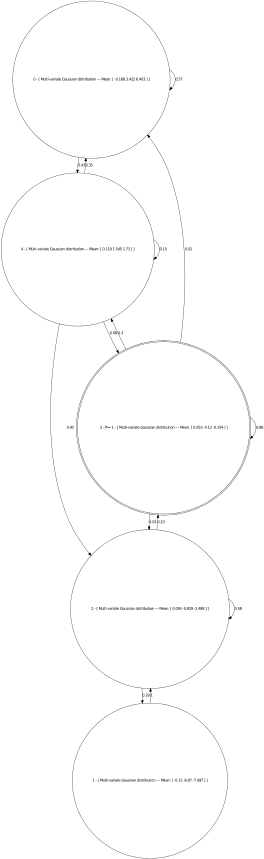
\includegraphics[scale=1.00]{00_resources/figures/output.png}
\caption{Hidden Markov Model}
\label{}
\end{figure}





